%! Author = Matthias
%! Date = 13.10.2020

% Preamble
\documentclass[11pt]{article}

% Packages
\usepackage{amsmath}
\usepackage{float}
\usepackage{graphicx}
\usepackage{gensymb}
\usepackage{mathtools}
\usepackage{fancyhdr}
\usepackage{german}

\pagestyle{fancy}
\fancyhf{}
\rhead{Matthias Rupp}
\lhead{Autonome Systeme - Bewegung}

% Document
\begin{document}
    \section{Hausaufgabe 1}\label{sec:home}
    Aufgabe: entwickeln Sie die Vorw"arts- und R"uckw"artskinematik des folgenden Roboters:
    \begin{figure}[H]
        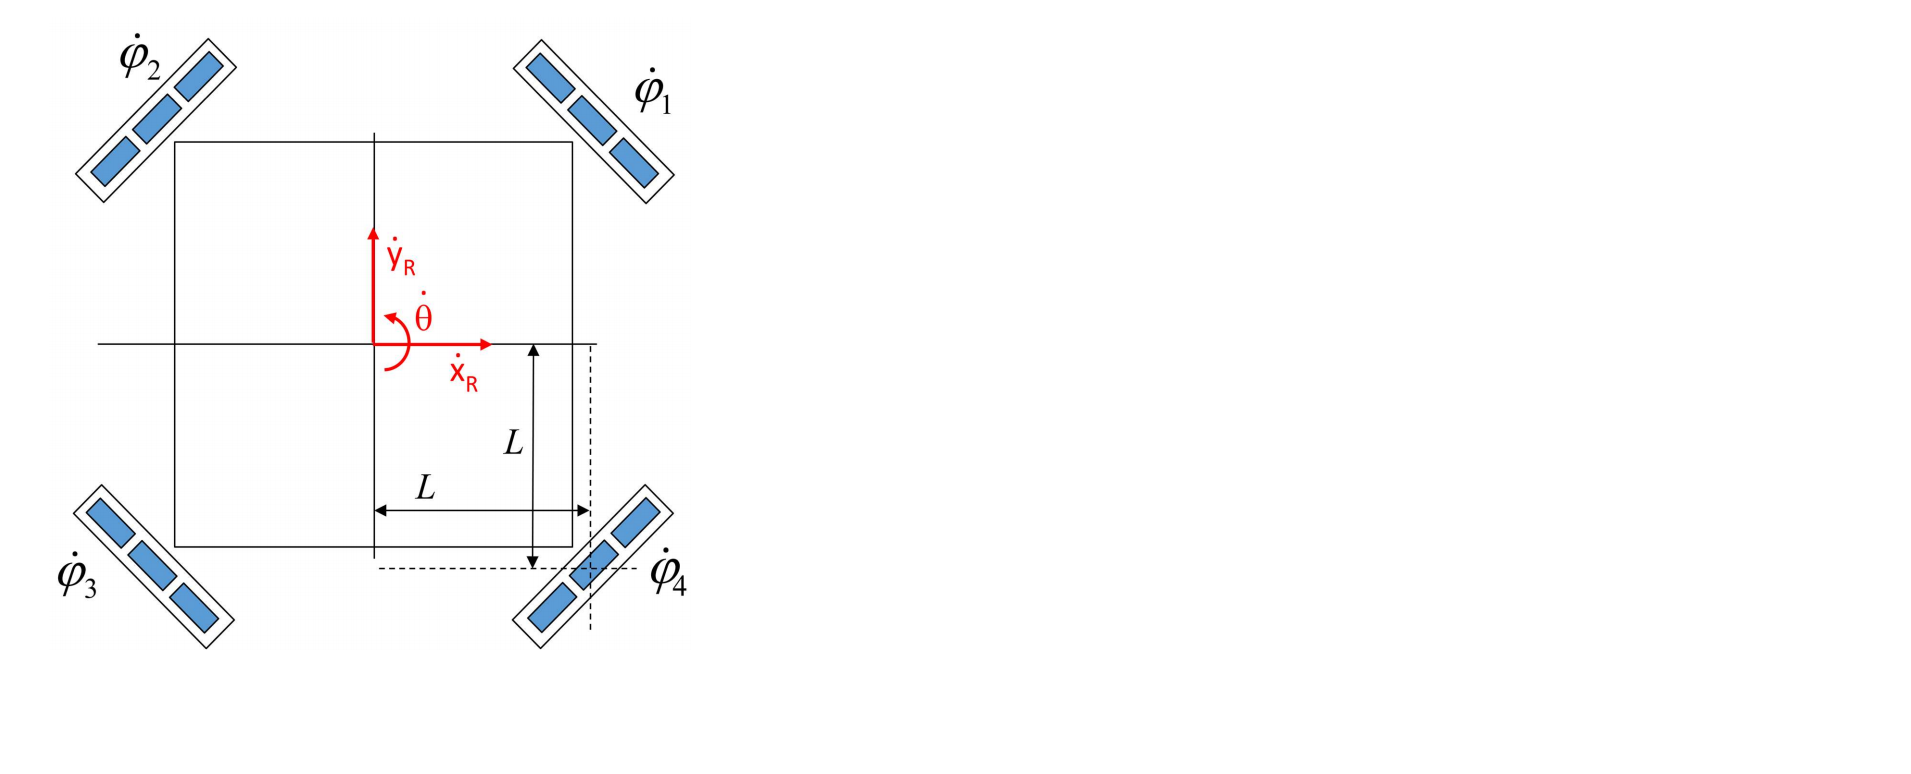
\includegraphics{../images/aufgabeDOriginal.png}
        \caption{Roboter}
        \label{fig:rob}
    \end{figure}

    \subsection{R"uckw"artskinematik}\label{subsubsec:ruck}
    Die Zwangsbedingung f"ur das Omni-wheel gleicht jener f"ur das Mecanum Wheel, mit der Ausnahme, dass der Winkel $\gamma$ null ist, da das Rad nicht im 45 Grad Winkel rotiert zur Fahrtrichtung steht.
    \begin{equation}
        \dot{x}_{R}\cos\left(  \gamma + \delta \right) - \dot{y}_{R}\sin\left( \gamma + \delta \right) - l \dot{\theta}\sin\left( \alpha + \gamma + \delta \right) = r\dot{\varphi}\cos\gamma\label{eq:zwang}
    \end{equation}
    Umgeformt (da $ \gamma $ gleich 0 und $ \cos\gamma $ gleich 1):
    \begin{equation}
        \dot{x}_{R}\cos\left(\delta \right) - \dot{y}_{R}\sin\left(\delta \right) - l \dot{\theta}\sin\left( \alpha + \delta \right) = r\dot{\varphi}\label{eq:zwangumgf}
    \end{equation}
    Der n"achste Schritt ist das Bestimmen der Winkel anhand der Zeichnung.
    \begin{figure}[H]
        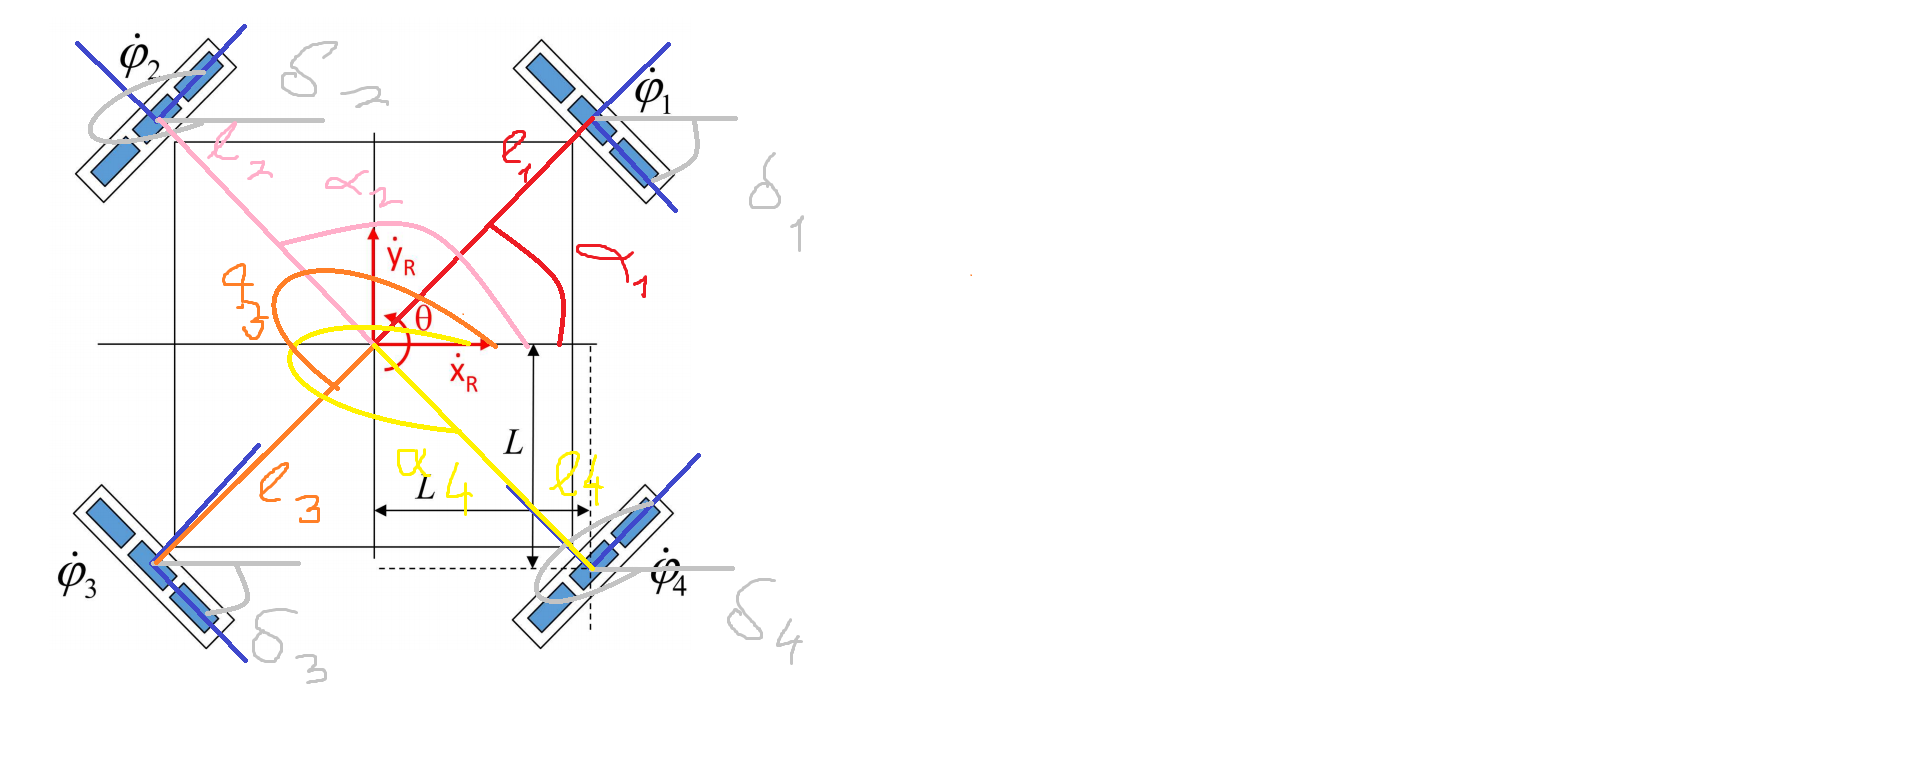
\includegraphics{../images/aufgabeDOriginalWinkelV2.png}
        \caption{Eingezeichnete Winkel}
        \label{fig:winkel}
    \end{figure}
    Im Anschluss, die Tabelle.
    \begin{table}[H]
        \begin{tabular}{|c|c|c|c|c|c}
            \hline
            i & $\alpha$                     & $\gamma$ & $\delta$      & l            \\ \hline
            1 & $\arctan(L/L)$               & 0        & $45\degree$   & $L*\sqrt{2}$ \\ \hline
            2 & $180\degree - \arctan(L/L)$  & 0        & $-45\degree$  & $L*\sqrt{2}$ \\ \hline
            3 & $-180\degree + \arctan(L/L)$ & 0        & $45\degree$ & $L*\sqrt{2}$ \\ \hline
            4 & $- \arctan(L/L)$             & 0        & $-45\degree$  & $L*\sqrt{2}$ \\ \hline
        \end{tabular}\caption{Tabelle der Winkel}\label{tab:winkeltab}
        \label{tab:winkeltabelle}
    \end{table}
    $L/L = 1$, also gilt fuer alle $\arctan$:\space$\arctan1 = 45\degree$.
    Die Werte f"ur $\alpha$ sind also ausgerechnet: $45\degree, 180\degree-45\degree = 135\degree, -180\degree+45 \degree = -135\degree, -45\degree$.
    Wir setzen nun in die Zwangsbedingung ein:
    \begin{equation}
        \dot{x}_{R}\cos\left(45\degree \right) - \dot{y}_{R}\sin\left(45\degree \right) - L*\sqrt{2}\dot{\theta}\sin\left( 45\degree + 45\degree \right) = r\dot{\varphi_{1}}\label{eq:einsetzen1}
    \end{equation}
    \begin{equation}
        \dot{x}_{R}\cos\left(-45\degree \right) - \dot{y}_{R}\sin\left(-45\degree \right) - L*\sqrt{2}\dot{\theta}\sin\left( 135\degree -45\degree \right) = r\dot{\varphi_{2}}\label{eq:einsetzen2}
    \end{equation}
    \begin{equation}
        \dot{x}_{R}\cos\left(45\degree \right) - \dot{y}_{R}\sin\left(45\degree \right) - L*\sqrt{2}\dot{\theta}\sin\left( -135\degree + 45\degree \right) = r\dot{\varphi_{3}}\label{eq:einsetzen3}
    \end{equation}
    \begin{equation}
        \dot{x}_{R}\cos\left(-45\degree \right) - \dot{y}_{R}\sin\left(-45\degree \right) - L*\sqrt{2}\dot{\theta}\sin\left( -45\degree - 45\degree \right) = r\dot{\varphi_{4}}\label{eq:einsetzen4}
    \end{equation}

    Ausgerechnet:
    \begin{equation}
        \dot{x}_{R}\sqrt{2}/2 - \dot{y}_{R}\sqrt{2}/2 - L*\sqrt{2}\dot{\theta} = r\dot{\varphi_{1}}\label{eq:calc1}
    \end{equation}
    \begin{equation}
        \dot{x}_{R}\sqrt{2}/2 + \dot{y}_{R}\sqrt{2}/2 - L*\sqrt{2}\dot{\theta} = r\dot{\varphi_{2}}\label{eq:calc2}
    \end{equation}
    \begin{equation}
        \dot{x}_{R}\sqrt{2}/2 - \dot{y}_{R}\sqrt{2}/2 + L*\sqrt{2}\dot{\theta} = r\dot{\varphi_{3}}\label{eq:calc3}
    \end{equation}
    \begin{equation}
        \dot{x}_{R}\sqrt{2}/2 + \dot{y}_{R}\sqrt{2}/2 + L*\sqrt{2}\dot{\theta} = r\dot{\varphi_{4}}\label{eq:calc4}
    \end{equation}
    Wenn man die Geschwindigkeiten in einem Vektor zusammenfasst, erh"alt man die R"uckw"artskinematik.
    \begin{equation}
        \begin{bmatrix}
            \dot{\varphi}_{1} \\
            \dot{\varphi}_{2} \\
            \dot{\varphi}_{3} \\
            \dot{\varphi}_{4} \\
        \end{bmatrix}\label{eq:rueck} = \frac{1}{r}
        \begin{bmatrix}
            \frac{\sqrt{2}}{2} & \frac{-\sqrt{2}}{2} & -L\sqrt{2} \\
            \frac{\sqrt{2}}{2} & \frac{\sqrt{2}}{2} & -L\sqrt{2} \\
            \frac{\sqrt{2}}{2} & \frac{-\sqrt{2}}{2} & L\sqrt{2} \\
            \frac{\sqrt{2}}{2} & \frac{\sqrt{2}}{2} & L\sqrt{2} \\
        \end{bmatrix}
        \begin{bmatrix}
            \dot{x}_{R} \\
            \dot{y}_{R} \\
            \dot{\theta} \\
        \end{bmatrix}
    \end{equation}
    Die inverse Jakobimatrix ist also:
    \begin{equation}
        \prescript{R}{}{J} = \frac{1}{r}
        \begin{bmatrix}
            \frac{\sqrt{2}}{2} & \frac{-\sqrt{2}}{2} & -L\sqrt{2} \\
            \frac{\sqrt{2}}{2} & \frac{\sqrt{2}}{2} & -L\sqrt{2} \\
            \frac{\sqrt{2}}{2} & \frac{-\sqrt{2}}{2} & L\sqrt{2} \\
            \frac{\sqrt{2}}{2} & \frac{\sqrt{2}}{2} & L\sqrt{2} \\
        \end{bmatrix}\label{eq:jakobi}
    \end{equation}

    \subsection{Berechnung der Vorw"artskinematik}\label{subsec:vor}
    F"ur die Vorw"artskinematik berechnet man die Invertierte der Jakobimatrix von (12).
    Hierbei ist zu bedenken, dass das Gleichungssystem mit den Winkelgeschwindigkeiten der 4 R"ader "uberbestimmt ist (da nur 3 Koordinatent im kartesischen Raum bestimmt werden sollen).
    3 R"ader sind hierf"ur ausreichend, das vierte Rad muss dann entsprechend den anderen R"adern eingestellt werden.
    Hierzu teilt man die Jakobimatrix in eine $J_{3}$, mit 3 Zeilen zur Festlegung der kartesischen Geschwindigkeiten und eine $J_{m}$, welche die Zwangsbedingung f"ur die Winkelgeschwindigkeit des vierten Rades vorgibt.
    \begin{equation}
        \prescript{R}{}{J}_{3} = \frac{1}{r}
        \begin{bmatrix}
            \frac{\sqrt{2}}{2} & \frac{-\sqrt{2}}{2} & -L\sqrt{2} \\
            \frac{\sqrt{2}}{2} & \frac{\sqrt{2}}{2} & -L\sqrt{2} \\
            \frac{\sqrt{2}}{2} & \frac{-\sqrt{2}}{2} & L\sqrt{2} \\
        \end{bmatrix}\label{eq:j3}
        \prescript{R}{}{J}_{m} = \frac{1}{r}
        \begin{bmatrix}
            \frac{\sqrt{2}}{2} & \frac{\sqrt{2}}{2} & L\sqrt{2} \\
        \end{bmatrix}
    \end{equation}
    Die invertierte Matrix lautet nun:
    \begin{equation}
        \prescript{3}{}{J}^{-1} =
        \begin{bmatrix}
            0 & \frac{\sqrt{2}r}{2} & \frac{\sqrt{2}r}{2} \\
            -\frac{\sqrt{2}r}{2} & \frac{\sqrt{2}r}{2} & 0 \\
            -\frac{\sqrt{2}r}{4L} & 0 & \frac{\sqrt{2}r}{4L} \\
        \end{bmatrix}\label{eq:invertedj3}
    \end{equation}
    F"ur die Geschwindigkeit bedeutet das:
    \begin{equation}
        \label{eq:finalforward}
        \prescript{R}{}{v}=
        \begin{bmatrix}
            \dot{x}_{R} \\
            \dot{y}_{R} \\
            \dot{\theta} \\
        \end{bmatrix}
        = \prescript{R}{}{J}^{-1}_{3}
        \begin{bmatrix}
            \dot{\varphi_{1}} \\
            \dot{\varphi_{2}} \\
            \dot{\varphi_{3}} \\
        \end{bmatrix}
        =
        \begin{bmatrix}
            0 & \frac{\sqrt{2}r}{2} & \frac{\sqrt{2}r}{2} \\
            -\frac{\sqrt{2}r}{2} & \frac{\sqrt{2}r}{2} & 0 \\
            -\frac{\sqrt{2}r}{4L} & 0 & \frac{\sqrt{2}r}{4L} \\
        \end{bmatrix}
        \begin{bmatrix}
            \dot{\varphi_{1}} \\
            \dot{\varphi_{2}} \\
            \dot{\varphi_{3}} \\
        \end{bmatrix}
    \end{equation}


\end{document}